\chapter{Experiments}


\begin{figure}[!hbt]
  \centering
  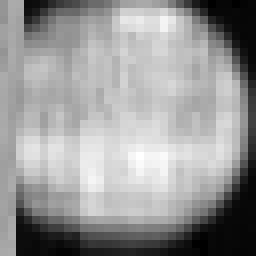
\includegraphics[width=4cm]{oil}
  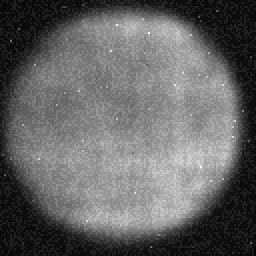
\includegraphics[width=4cm]{water}
  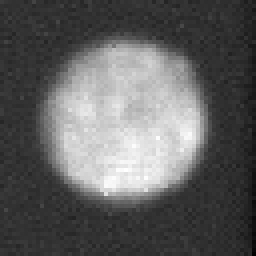
\includegraphics[width=4cm]{air}
  \caption{dfaxs}
  \label{fig:immersion-bfp-scan}
\end{figure}

\begin{figure}[!hbt]
  \centering
  \input{tirf-exp.eps_tex} 
  \caption{A fluorescent plane on a slide is embedded in oil, water or
    air. The thickness of the embedding medium is approximately
    $\unit[5]{\mu m}$. The LCoS illuminates a disk with $\unit[30]{\mu
      m}$ diameter while a $14\times 14$ window is scanned over the
    MMA.}
  \label{fig:tirf-exp}
\end{figure}

